\documentclass[aspectratio=169,11pt]{beamer}

\usepackage[T1]{fontenc}
\usepackage{mathpazo}
\usepackage{geometry}
\geometry{paperwidth=19.2cm,paperheight=10.8cm}
\usepackage{graphicx}
\usepackage{sourcesanspro}
\usepackage{inconsolata}
\usepackage{tikz}
\usepackage{booktabs}
\usepackage{amsmath,amssymb}
\usepackage{tcolorbox}
\usepackage{listings}
\usepackage{array}
\usetikzlibrary{arrows.meta,positioning,trees,decorations.pathmorphing}

\renewcommand{\familydefault}{\sfdefault}
\overfullrule=0pt

% ---------- palette ----------
\definecolor{paper}{HTML}{FAF9F4}
\definecolor{ink}{HTML}{20242A}
\definecolor{inkdim}{HTML}{5C6058}
\definecolor{accent}{HTML}{8B6914}
\definecolor{accentB}{HTML}{1F6F68}
\definecolor{neg}{HTML}{A24A3B}
\definecolor{panel}{HTML}{F1EFE6}
\definecolor{linecol}{HTML}{D8D5C9}

% ---------- beamer stripping ----------
\setbeamertemplate{navigation symbols}{}
\setbeamercolor{background canvas}{bg=paper}
\setbeamercolor{normal text}{fg=ink,bg=paper}
\setbeamercolor{structure}{fg=accent}
\setbeamertemplate{itemize item}{\color{accentB}\textbullet}
\setbeamertemplate{itemize subitem}{\color{inkdim}\textendash}
\setbeamerfont{itemize/enumerate body}{size=\normalsize}
\setlength{\parskip}{5pt}

\setbeamertemplate{footline}{%
  \leavevmode%
  \hbox{\begin{beamercolorbox}[wd=\paperwidth,ht=3.6ex,dp=1.8ex,leftskip=18pt,rightskip=18pt]{footline}%
    {\scriptsize\sffamily\color{inkdim}From MDPs to GRPO}%
    \hfill
    {\scriptsize\ttfamily\color{inkdim}\insertframenumber\,/\,\inserttotalframenumber}%
  \end{beamercolorbox}}%
}
\setbeamercolor{footline}{bg=paper,fg=inkdim}

% ---------- code listing style ----------
\lstset{
  basicstyle=\ttfamily\footnotesize\color{ink},
  commentstyle=\itshape\color{inkdim},
  keywordstyle=\color{accentB},
  backgroundcolor=\color{panel},
  frame=single,
  rulecolor=\color{linecol},
  framerule=0.5pt,
  showstringspaces=false,
  breaklines=true,
  xleftmargin=12pt,
  framexleftmargin=10pt,
  morecomment=[l]{\#},
  aboveskip=6pt,
  belowskip=4pt,
}

% ---------- custom components ----------
\newcommand{\eyebrow}[2]{%
  \noindent{\scriptsize\sffamily\color{inkdim}\MakeUppercase{#1}}\hfill{\scriptsize\ttfamily\color{accentB}#2}\\[3pt]
  {\color{linecol}\rule{\linewidth}{0.6pt}}\\[13pt]%
}
\newcommand{\headline}[1]{{\usefont{T1}{ppl}{b}{n}\selectfont\LARGE\color{ink} #1}\par\vspace{10pt}}
\newcommand{\lede}[1]{{\normalsize\color{inkdim} #1}\par\vspace{6pt}}
\newcommand{\frametag}[2]{{\small\sffamily\bfseries\color{#1}\MakeUppercase{#2}}\par\vspace{4pt}}
\newcommand{\swatch}[1]{\textcolor{#1}{\rule{7pt}{7pt}}}

\newtcolorbox{eqbox}[1][]{%
  colback=panel,colframe=linecol,boxrule=0.6pt,arc=3pt,
  left=16pt,right=16pt,top=8pt,bottom=8pt,
  halign=center,#1
}
\newtcolorbox{eqboxhi}[1][]{%
  colback=panel,colframe=accent,boxrule=0.8pt,arc=3pt,
  left=16pt,right=16pt,top=8pt,bottom=8pt,
  halign=center,#1
}
\newtcolorbox{callout}[1][]{%
  colback=panel,colframe=accentB,boxrule=0pt,leftrule=3pt,arc=0pt,
  left=13pt,right=13pt,top=7pt,bottom=7pt,#1
}
\newtcolorbox{calloutwarm}[1][]{%
  colback=panel,colframe=accent,boxrule=0pt,leftrule=3pt,arc=0pt,
  left=13pt,right=13pt,top=7pt,bottom=7pt,#1
}
\newcommand{\clabel}[2]{{\small\sffamily\bfseries\color{#1}\MakeUppercase{#2}}\\[4pt]}

\newtcolorbox{card}[1][]{%
  colback=panel,colframe=linecol,boxrule=0.6pt,arc=2pt,
  left=11pt,right=11pt,top=9pt,bottom=9pt,valign=top,height=3.15cm,
  before upper=\raggedright,#1
}
\newtcolorbox{cardA}[1][]{%
  colback=panel,colframe=accent,boxrule=0.8pt,arc=2pt,
  left=11pt,right=11pt,top=9pt,bottom=9pt,valign=top,height=3.15cm,
  before upper=\raggedright,#1
}
\newtcolorbox{cardB}[1][]{%
  colback=panel,colframe=accentB,boxrule=0.8pt,arc=2pt,
  left=11pt,right=11pt,top=9pt,bottom=9pt,valign=top,height=3.15cm,
  before upper=\raggedright,#1
}

\newcommand{\trajdiagram}{%
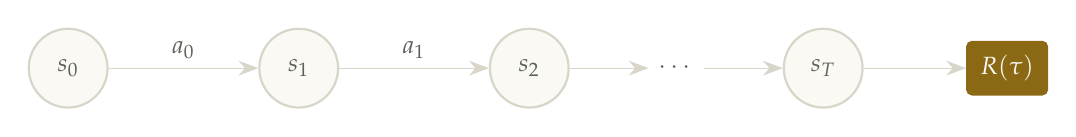
\begin{tikzpicture}[baseline,node distance=19mm]
  \tikzstyle{st}=[circle,draw=linecol,thick,minimum size=10mm,font=\small\ttfamily,fill=paper,text=inkdim]
  \tikzstyle{rw}=[rectangle,rounded corners=2pt,draw=accent,fill=accent,text=paper,font=\small\sffamily\bfseries,inner sep=5pt]
  \node[st] (s0) {$s_0$};
  \node[st,right=of s0] (s1) {$s_1$};
  \node[st,right=of s1] (s2) {$s_2$};
  \node[right=10mm of s2,inkdim] (dots) {\ttfamily\small $\cdots$};
  \node[st,right=10mm of dots] (sT) {$s_T$};
  \node[rw,right=13mm of sT] (r) {$R(\tau)$};
  \draw[-{Stealth[length=2.5mm]},linecol] (s0) -- node[above,font=\small\ttfamily,color=inkdim]{$a_0$} (s1);
  \draw[-{Stealth[length=2.5mm]},linecol] (s1) -- node[above,font=\small\ttfamily,color=inkdim]{$a_1$} (s2);
  \draw[-{Stealth[length=2.5mm]},linecol] (s2) -- (dots);
  \draw[-{Stealth[length=2.5mm]},linecol] (dots) -- (sT);
  \draw[-{Stealth[length=2.5mm]},linecol] (sT) -- (r);
\end{tikzpicture}}

\begin{document}

% ================= 01 : COVER MEME =================
\begin{frame}[c]
\begin{center}
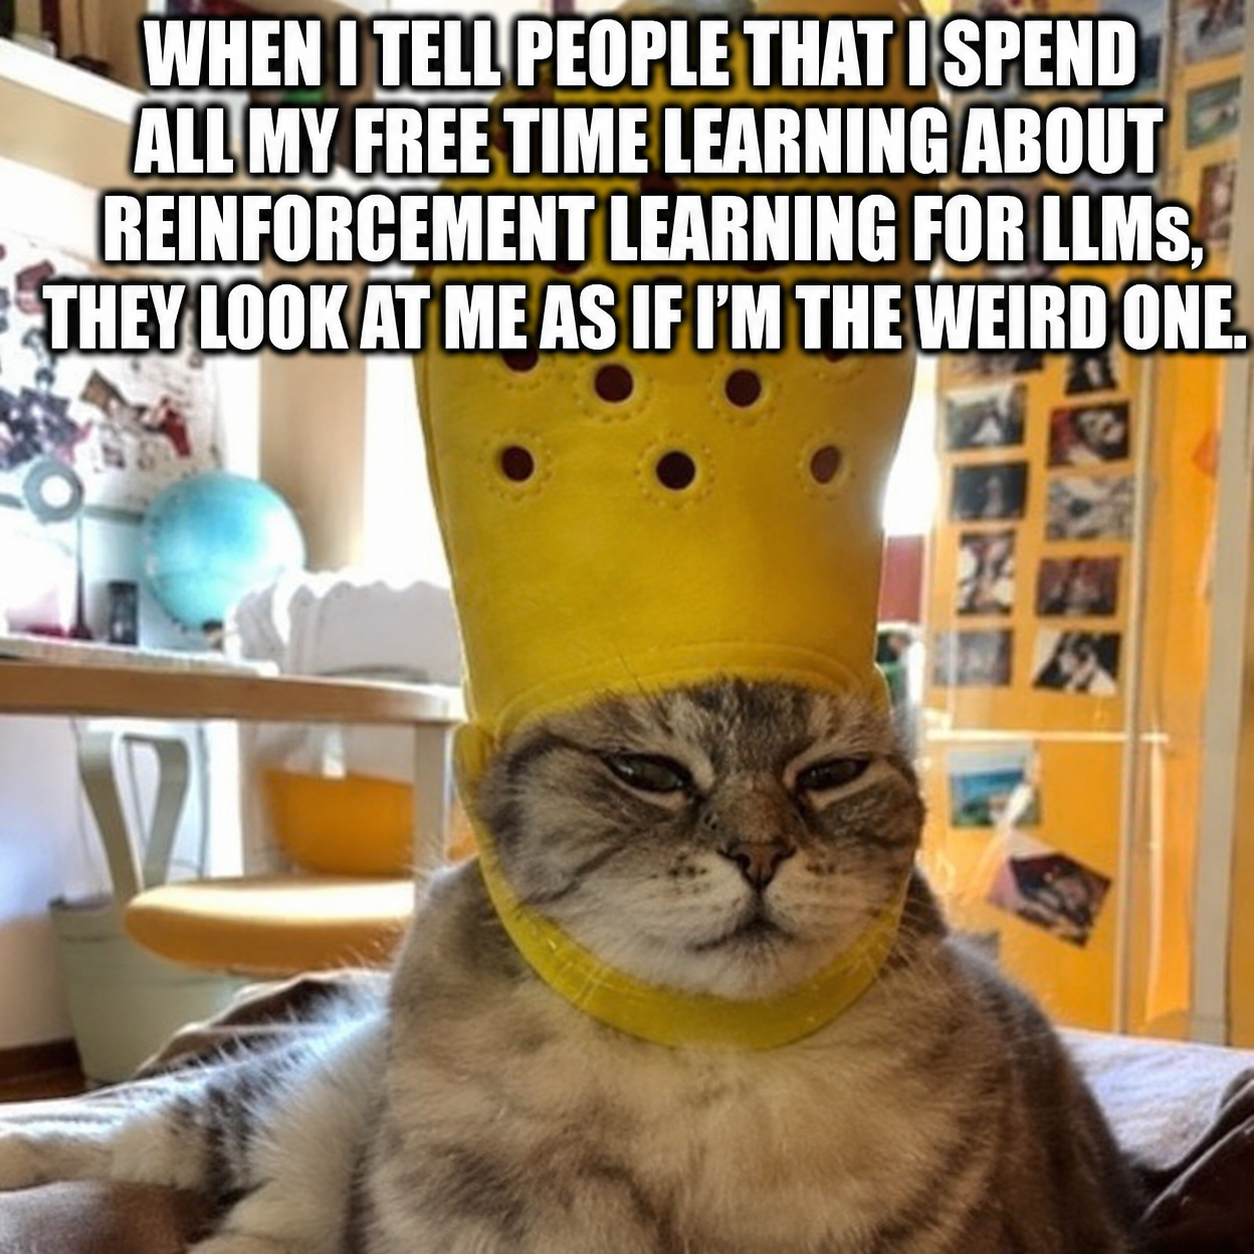
\includegraphics[height=8.6cm]{cover-meme.png}
\end{center}
\end{frame}

% ================= 02 : TITLE =================
\begin{frame}
\eyebrow{Framing \textperiodcentered\ 02}{}
\vspace{8pt}
{\usefont{T1}{ppl}{b}{n}\selectfont\Huge\color{ink} From MDPs to \textcolor{accent}{\textit{GRPO}}}\par
\vspace{18pt}
{\Large\color{inkdim} Four problems, four fixes: how reinforcement learning becomes a training signal for a language model, and how each limitation of one method motivates the next.}
\par\vspace{28pt}
\trajdiagram
\par\vspace{14pt}
{\small\color{inkdim} Every intermediate node is silent. The only lit node is the last one --- that single fact drives most of what follows.}
\end{frame}

% ================= 02 : THE CHAIN =================
\begin{frame}
\eyebrow{Framing \textperiodcentered\ 03}{}
\headline{One idea leads to the next}
\small
\renewcommand{\arraystretch}{1.05}
\begin{tabular}{@{} >{\raggedright\arraybackslash}p{2.6cm} p{13.6cm} @{}}
{\bfseries\color{neg}Problem} & Reward only appears at the very end of a response. \\
{\bfseries\color{accentB}Approach} & \textbf{Policy gradients} --- reinforce every token in a trajectory that scored well. \\[2pt]
{\bfseries\color{neg}Problem} & ``Good'' is meaningless without something to compare it to. \\
{\bfseries\color{accentB}Approach} & \textbf{Proximal Policy Optimization (PPO)} --- score against a learned value baseline; clip large updates. \\[2pt]
{\bfseries\color{neg}Problem} & That value baseline is a whole second network to train. \\
{\bfseries\color{accentB}Approach} & \textbf{Group Relative Policy Optimization (GRPO)} --- score completions against each other instead. \\[2pt]
{\bfseries\color{neg}Problem} & A reward model still needs human-labeled preference data. \\
{\bfseries\color{accentB}Approach} & \textbf{Reinforcement Learning with Verifiable Rewards (RLVR)} --- let a deterministic checker score it. \\[2pt]
{\bfseries\color{accent}Result} & DeepSeek-R1-Zero reasons well but reads poorly --- DeepSeek-R1 stages that into a usable model. \\
\end{tabular}
\end{frame}

% ================= 03 : CLASSICAL MDP DEFS =================
\begin{frame}
\eyebrow{Classical MDP \textperiodcentered\ 04}{background}
\headline{The vocabulary reinforcement learning starts with}
\lede{A \textbf{Markov Decision Process (MDP)} is the tuple $(S,A,P,R,\gamma)$. Everything else in this deck is a choice about how to fill in these six ideas.}
\vspace{6pt}
\begin{tabular}{@{} l p{13cm} @{}}
\toprule
\textbf{\small SYMBOL} & \textbf{\small MEANING} \\
\midrule
\color{accentB}$s \in S$ & State --- everything the agent currently knows. \\
\color{accentB}$a \in A$ & Action --- a choice available from that state. \\
\color{accentB}$P(s'\mid s,a)$ & Transition --- how the environment responds. \\
\color{accentB}$r = R(s,a,s')$ & Reward --- the scalar signal returned by the environment. \\
\color{accentB}$\pi(a\mid s)$ & Policy --- the agent's rule for choosing actions. \\
\color{accentB}$\gamma \in [0,1]$ & Discount --- how much future reward counts right now. \\
\bottomrule
\end{tabular}
\end{frame}

% ================= 04 : MDP AS A GRAPH =================
\begin{frame}
\eyebrow{Classical MDP \textperiodcentered\ 05}{background}
\headline{What that tuple actually looks like}
\begin{center}
\scalebox{0.82}{
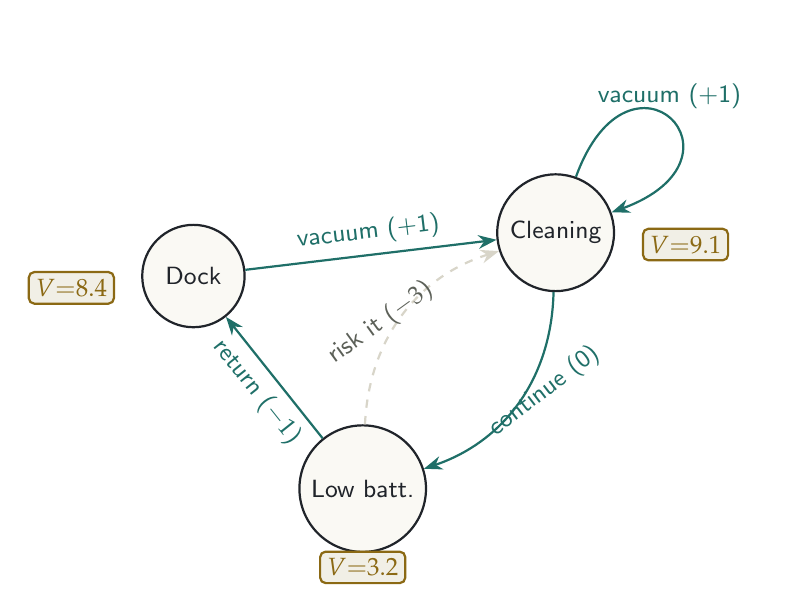
\begin{tikzpicture}[>=Stealth]
 \tikzstyle{mdpstate}=[circle,draw=ink,thick,minimum size=13mm,font=\small\sffamily,fill=paper,text=ink]
 \tikzstyle{vtag}=[rectangle,rounded corners=2pt,draw=accent,thick,fill=panel,font=\small\ttfamily,text=accent,inner sep=2.5pt]
 \node[mdpstate] (dock) at (0,0) {Dock};
 \node[mdpstate] (clean) at (4.6,0.55) {Cleaning};
 \node[mdpstate] (low) at (2.15,-2.7) {Low batt.};
 \node[vtag] at (-1.55,-0.15) {$V{=}8.4$};
 \node[vtag] at (6.25,0.4) {$V{=}9.1$};
 \node[vtag] at (2.15,-3.7) {$V{=}3.2$};
 \draw[->,accentB,thick] (dock) -- node[above,font=\small\sffamily,sloped]{vacuum (+1)} (clean);
 \draw[->,accentB,thick] (clean) to[out=70,in=20,looseness=8] node[above,font=\small\sffamily]{vacuum (+1)} (clean);
 \draw[->,accentB,thick] (clean) to[bend left=35] node[pos=0.72,right,font=\small\sffamily,sloped]{continue (0)} (low);
 \draw[->,accentB,thick] (low) -- node[below,font=\small\sffamily,sloped]{return ($-1$)} (dock);
 \draw[->,linecol,thick,dashed] (low) to[bend left=35] node[pos=0.72,left,font=\small\sffamily,sloped,color=inkdim]{risk it ($-3$)} (clean);
\end{tikzpicture}
}
\end{center}
{\small\color{ink}Circles are states $s$, each carrying its value $V^\pi(s)$. Arrows are transitions under $\pi$, labeled with the action and reward. From \textit{Low battery}, the policy prefers \textit{return} over \textit{risk it} because it leads toward the higher-value state.}
\end{frame}

% ================= 05 : VALUE FUNCTIONS =================
\begin{frame}
\eyebrow{Classical MDP \textperiodcentered\ 06}{background}
\headline{The classical move: estimate value, then improve}
\begin{eqbox}[fontupper=\normalsize]
$V^\pi(s) = \mathbb{E}_\pi\big[\sum_{k=0}^{\infty}\gamma^k r_{t+k} \mid s_t=s\big]$ \\[6pt]
$Q^\pi(s,a) = \mathbb{E}_\pi\big[\sum_{k=0}^{\infty}\gamma^k r_{t+k} \mid s_t=s,\,a_t=a\big]$
\end{eqbox}
\vspace{8pt}
{\normalsize\color{ink} Classical RL usually assumes reward is available at, or near, every step --- so value can be \textit{bootstrapped}: propagated backward without waiting for an episode to end.}
\par\vspace{8pt}
\begin{callout}
\clabel{accentB}{Where your prior picture came from}
{\small\color{ink}Dynamic programming, TD-learning, ordinary actor--critic --- all of them lean on dense, per-step feedback. That's exactly the assumption LLM training breaks.}
\end{callout}
\end{frame}

% ================= 06 : MAPPING TO LLM =================
\begin{frame}
\eyebrow{LLM as MDP \textperiodcentered\ 07}{\S7.1}
\headline{Same tuple, new content}
\lede{Token generation is still an ordinary episodic MDP. Only what fills each slot changes.}
\begin{tabular}{@{} l p{13cm} @{}}
\toprule
\textbf{\small MDP SLOT} & \textbf{\small LLM INSTANTIATION} \\
\midrule
\color{accentB}$s_t$ & Prompt + tokens generated so far: $(x, y_1,\dots,y_{t-1})$ \\
\color{accentB}$a_t$ & The next sampled token, $y_t$ \\
\color{accentB}$P$ & Deterministic append: $s_{t+1} = (s_t, a_t)$ \\
\color{accentB}$\pi_\theta$ & The model's own next-token distribution --- its weights \textit{are} the policy \\
\color{accentB}$T$ & Episode length --- until an end token or a length cap \\
\bottomrule
\end{tabular}
\par\vspace{10pt}
{\normalsize\color{ink}During rollouts we sample from this distribution rather than taking argmax. Sampling is what makes exploration possible.}
\end{frame}

% ================= 07 : PROBLEM -- SPARSE REWARD =================
\begin{frame}
\eyebrow{LLM as MDP \textperiodcentered\ 08}{\S7.1.3}
\frametag{neg}{Problem}
\headline{Reward only shows up at the very end}
\begin{eqbox}
$r_1 = r_2 = \cdots = r_{T-1} = 0, \quad r_T = R(\tau)$
\end{eqbox}
\vspace{6pt}
\centerline{\trajdiagram}
\par\vspace{8pt}
{\small\color{ink}A verifier scores the \textit{finished} response, not each token. Every token in a completion shares that one terminal reward, so credit assignment is crude: the model can't tell which specific token deserved it.}
\par\vspace{8pt}
\begin{calloutwarm}
\clabel{accent}{Key distinction}
{\small\color{ink}This is the real gap from classical RL: not a different \textit{kind} of problem, but one where the reward almost never shows up until the very end of the episode.}
\end{calloutwarm}
\end{frame}

% ================= 08 : LLM AS A TREE =================
\begin{frame}
\eyebrow{LLM as MDP \textperiodcentered\ 09}{}
\headline{The same picture, redrawn for a language model}
\begin{center}
\scalebox{1.05}{
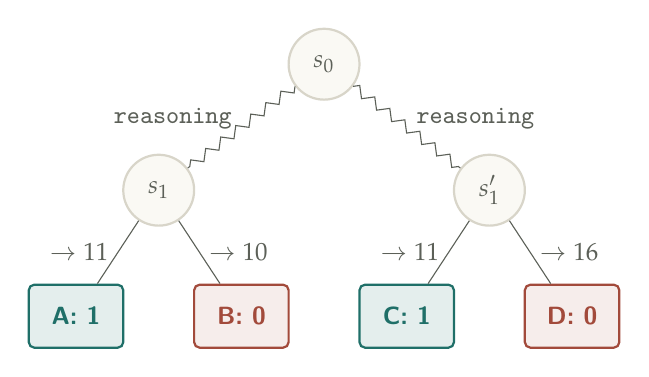
\begin{tikzpicture}[
  level 1/.style={sibling distance=42mm,level distance=16mm},
  level 2/.style={sibling distance=21mm,level distance=16mm},
  st/.style={circle,draw=linecol,thick,minimum size=9mm,fill=paper,text=inkdim,font=\small\ttfamily},
  leafgood/.style={rectangle,rounded corners=2pt,draw=accentB,thick,fill=accentB!12,minimum width=12mm,minimum height=8mm,font=\small\sffamily\bfseries,text=accentB},
  leafbad/.style={rectangle,rounded corners=2pt,draw=neg,thick,fill=neg!10,minimum width=12mm,minimum height=8mm,font=\small\sffamily\bfseries,text=neg},
  edgelab/.style={font=\small\ttfamily,color=inkdim,midway},
  manytoken/.style={decorate,decoration={zigzag,segment length=2.4mm,amplitude=0.6mm},draw=inkdim}
]
\node[st] {$s_0$}
  child { node[st] {$s_1$}
    child { node[leafgood] {A: 1} edge from parent node[edgelab,left]{$\to 11$} }
    child { node[leafbad] {B: 0} edge from parent node[edgelab,right]{$\to 10$} }
    edge from parent[manytoken] node[edgelab,left,yshift=3pt]{reasoning}
  }
  child { node[st] {$s_1'$}
    child { node[leafgood] {C: 1} edge from parent node[edgelab,left]{$\to 11$} }
    child { node[leafbad] {D: 0} edge from parent node[edgelab,right]{$\to 16$} }
    edge from parent[manytoken] node[edgelab,right,yshift=3pt]{reasoning}
  };
\end{tikzpicture}
}
\end{center}
{\small\color{ink}No cycles, no self-loops --- each token choice is a branch, never a return, and no node carries a $V(s)$ the way \textit{Dock} or \textit{Cleaning} did. The wavy edges each compress \textit{many} single-token states into one arrow; only the short straight edge into each leaf is one real token. Reward (green/red) exists only at the leaves.}
\end{frame}

% ================= 09 : BLOCK 1 -- J(THETA) =================
\begin{frame}
\eyebrow{Building Blocks \textperiodcentered\ 10}{\S7.2}
\frametag{inkdim}{Building block 1}
\headline{What are we even trying to maximize?}
\begin{eqbox}[fontupper=\normalsize]
$J(\theta) = \mathbb{E}_{x\sim D}\,\mathbb{E}_{y\sim\pi_\theta(\cdot|x)}\big[R(x,y)\big]$
\end{eqbox}
\par\vspace{10pt}
{\normalsize\color{ink}$J(\theta)$ is the average reward we'd get if we sampled forever from the current model, across the training prompts. Maximizing $J(\theta)$ means: make good responses more likely, bad ones less likely.}
\par\vspace{10pt}
\begin{callout}
\clabel{accentB}{Why the letter $J$}
{\small\color{ink}There's no hidden meaning --- $J$ is just conventional RL notation for an objective function: ``the quality of the policy parameterized by $\theta$.'' Everything from here on is a piece we'll use to climb $J(\theta)$.}
\end{callout}
\end{frame}

% ================= 10 : BLOCK 2 -- MONTE CARLO =================
\begin{frame}
\eyebrow{Building Blocks \textperiodcentered\ 11}{\S7.2}
\frametag{inkdim}{Building block 2}
\headline{Estimating its gradient from sampled rollouts}
{\normalsize\color{ink}We can't compute $J(\theta)$ exactly --- the space of possible completions is astronomically large. So instead of the true gradient, we estimate it using a handful of actual sampled rollouts. That's a \textbf{Monte Carlo} estimate: approximate an average using samples instead of the full computation.}
\par\vspace{10pt}
\begin{eqbox}[fontupper=\normalsize]
$\nabla_\theta J(\theta) \;\approx\; \dfrac{1}{N}\displaystyle\sum_{i=1}^{N} R(\tau_i)\sum_{t}\nabla_\theta\log\pi_\theta(a_{i,t}\mid s_{i,t})$
\end{eqbox}
\par\vspace{10pt}
\begin{callout}
\clabel{accentB}{Why this is allowed}
{\small\color{ink}This estimate is unbiased for \textit{any} $N$, including $N{=}1$ --- that's what licenses training on a small sampled batch instead of the intractable full sum.}
\end{callout}
\end{frame}

% ================= 11 : BLOCK 3 -- ONE TOKEN =================
\begin{frame}
\eyebrow{Building Blocks \textperiodcentered\ 12}{\S7.2.2}
\frametag{inkdim}{Building block 3}
\headline{Zooming into a single sampled token}
{\normalsize\color{ink}Drop the sums over samples and time, and look at what happens to just one token. This is the piece both PPO and GRPO are built on:}
\par\vspace{8pt}
\begin{eqboxhi}[fontupper=\normalsize]
$\theta \;\leftarrow\; \theta + \alpha\,\underbrace{\nabla_\theta\log\pi_\theta(a_t\mid s_t)}_{\text{\swatch{accentB}\ token-level piece}}\,R$
\end{eqboxhi}
\par\vspace{10pt}
{\small\color{ink}$\alpha$ is the learning rate; the gradient term points toward higher probability for the token actually sampled; $R$ scales how hard to push, and in which direction. Sum this over every token in a response for the full update.}
\end{frame}

% ================= 12 : PROBLEM -- NOISY REWARD =================
\begin{frame}
\eyebrow{Baselines \& PPO \textperiodcentered\ 13}{\S7.2.3}
\frametag{neg}{Problem}
\headline{Reward alone can't tell you if an action was good}
{\normalsize\color{ink}Two prompts: an easy one where most completions score 1, a hard one where most score 0. A completion scoring 1 on the easy prompt may be unremarkable; a completion scoring 0 on the hard prompt may be one of the better attempts made. Raw $R(\tau)$ can't express ``good, relative to what this prompt usually produces.''}
\par\vspace{12pt}
\begin{eqbox}
$A_k = R_k - \text{baseline}(s_k)$
\end{eqbox}
\par\vspace{10pt}
\begin{callout}
\clabel{accentB}{The question every approach below answers differently}
{\small\color{ink}PPO and GRPO are, at heart, two different answers to one question: what should $\text{baseline}(s)$ actually be? Once we know, $R$ in block 3 gets replaced by this advantage $A$.}
\end{callout}
\end{frame}

% ================= 12b : BASELINE VARIANCE REDUCTION =================
\begin{frame}
\eyebrow{Baselines \& PPO \textperiodcentered\ 14}{\S7.2.3}
\headline{The baseline's real job: shrinking noise, not fixing bias}
{\footnotesize\color{ink}Two prompts of very different difficulty --- ``What is $12\times 3$?'' (easy) and ``Prove $\sqrt{2}$ is irrational'' (hard). Pool a batch of rollouts from both:}
\par\vspace{3pt}
\footnotesize
\begin{tabular}{@{} l l l l @{}}
\toprule
\textbf{Prompt} & \textbf{Reward $R$} & \textbf{baseline$(s)$} & \textbf{$A=R-\text{baseline}(s)$} \\
\midrule
Easy ($12\times3$) & 1 & 0.8 & $+0.2$ \\
Easy ($12\times3$) & 1 & 0.8 & $+0.2$ \\
Hard ($\sqrt2$ irrational) & 0 & 0.2 & $-0.2$ \\
Hard ($\sqrt2$ irrational) & 0 & 0.2 & $-0.2$ \\
\bottomrule
\end{tabular}
\par\vspace{3pt}
{\footnotesize\color{ink}Raw reward across the batch: mean $0.5$, variance $0.25$ --- almost entirely explained by \textit{which prompt} a completion came from, not how good it was. Baseline-adjusted advantage: mean $0$, variance $0.04$ --- $6.25\times$ smaller, since subtracting each prompt's typical score cancels the difficulty gap.}
\par\vspace{3pt}
\begin{callout}[top=4pt,bottom=4pt]
\clabel{accentB}{Same target, less noise}
{\footnotesize\color{ink}Raw $R$ and baseline-adjusted $A$ push the gradient the same direction on average --- subtracting a state-only function never biases it. But a batch dominated by prompt-difficulty swings teaches the model far less per rollout than one where that swing is already gone. That's the case for bothering with $\text{baseline}(s)$.}
\end{callout}
\end{frame}

% ================= 13 : BLOCK 4 -- KL DIVERGENCE =================
\begin{frame}
\eyebrow{Building Blocks \textperiodcentered\ 15}{}
\frametag{inkdim}{Building block 4}
\headline{Keeping the model close to a reference}
{\normalsize\color{ink}$\pi_\theta$ isn't a distribution --- it's a function from states to distributions. But fix one specific state $s_t$, and both $\pi_\theta(\cdot|s_t)$ and $\pi_{\text{ref}}(\cdot|s_t)$ become two ordinary, comparable distributions over the same vocabulary. \textbf{That} is what KL divergence compares.}
\par\vspace{8pt}
\begin{eqbox}[fontupper=\normalsize]
$\mathrm{KL}_t \;=\; \mathrm{KL}\big(\pi_\theta(\cdot\mid s_t)\,\Vert\,\pi_{\text{ref}}(\cdot\mid s_t)\big)$
\end{eqbox}
\par\vspace{10pt}
\begin{callout}
\clabel{accentB}{Computed how, in practice}
{\small\color{ink}Per token, reusing only the sampled token's probability under each model --- the same two numbers used for the ratio below --- via a low-variance single-sample estimator, not a full sum over the vocabulary.}
\end{callout}
\end{frame}

% ================= 14 : BRIDGE A -- WHY A REWRITE =================
\begin{frame}
\eyebrow{Baselines \& PPO \textperiodcentered\ 16}{\S7.3}
\headline{Why PPO needs a rewrite, not just the raw gradient}
{\normalsize\color{ink}Rollouts are expensive, so PPO takes \textit{several} gradient steps on the same batch before sampling again. But block 3's gradient is only valid at the exact $\theta$ that generated the data --- the moment $\theta$ moves, it stops being correct for this data. The fix is \textbf{importance sampling}: reweight old samples to estimate an expectation under the new policy.}
\par\vspace{8pt}
\begin{eqbox}[fontupper=\normalsize,top=6pt,bottom=6pt]
$\mathbb{E}_{a\sim\pi_\theta}\big[A(s,a)\big] \;=\; \mathbb{E}_{a\sim\pi_{\text{old}}}\Big[\dfrac{\pi_\theta(a\mid s)}{\pi_{\text{old}}(a\mid s)}\cdot A(s,a)\Big]$
\end{eqbox}
\par\vspace{8pt}
\begin{calloutwarm}
\clabel{accent}{Why reuse is even legitimate --- not in the book}
{\small\color{ink}A sampled token isn't owned by the policy that produced it --- any policy assigning it nonzero probability could have generated it. So after $\theta$ moves, the same recorded token is still valid data; we just ask how likely the \textit{current} policy thinks it was, and reweight by the ratio. \S7.3 presents the ratio as a stabilizer without explaining why reusing old samples this way is sound.}
\end{calloutwarm}
\end{frame}

% ================= 15 : BRIDGE B -- SAME GRADIENT =================
\begin{frame}
\eyebrow{Baselines \& PPO \textperiodcentered\ 17}{\S7.3}
\headline{The ratio is block 3's gradient, in disguise}
\small
\renewcommand{\arraystretch}{1.4}
\begin{tabular}{@{} l l @{}}
$\nabla_\theta\big[\text{ratio}_t(\theta)\cdot A_t\big] = \nabla_\theta\Big[\dfrac{\pi_\theta(a_t|s_t)}{\pi_{\text{old}}(a_t|s_t)}\Big]\cdot A_t$ & {\itshape\color{inkdim}differentiate the ratio; $\pi_{\text{old}}$ is fixed} \\
$= \dfrac{\pi_\theta(a_t|s_t)}{\pi_{\text{old}}(a_t|s_t)}\cdot\nabla_\theta\log\pi_\theta(a_t|s_t)\cdot A_t$ & {\itshape\color{inkdim}identity $\nabla f = f\cdot\nabla\log f$, again} \\
\end{tabular}
\par\vspace{6pt}
\begin{eqboxhi}[fontupper=\normalsize]
\text{at } $\theta=\theta_{\text{old}}$: \; $\text{ratio}_t=1 \;\Longrightarrow\; \nabla_\theta L(\theta)\big|_{\theta_{\text{old}}} = \nabla_\theta\log\pi_\theta(a_t|s_t)\cdot A_t$
\end{eqboxhi}
\par\vspace{10pt}
\begin{callout}
\clabel{accentB}{Why bother, if they agree at the start}
{\small\color{ink}Because $L(\theta)$ stays valid \textit{after} $\theta$ has moved a few steps --- you can keep differentiating it for several updates on the same batch. And $\text{ratio}_t(\theta)$ has a readable meaning (``how much more or less likely is this action now?''), so it can be directly clipped. That clip is the \textit{P} in Proximal.}
\end{callout}
\end{frame}

% ================= 16 : PROBLEM -- TRUST REGION NEEDED =================
\begin{frame}
\eyebrow{Baselines \& PPO \textperiodcentered\ 18}{\S7.3}
\frametag{neg}{Problem}
\headline{Exact in principle, unreliable in practice}
{\normalsize\color{ink}The identity behind the rewrite --- $\mathbb{E}_{\pi_\theta}[A] = \mathbb{E}_{\pi_{\text{old}}}[\text{ratio}_t(\theta)\cdot A]$ --- is exact for \textit{any} $\theta$; it never breaks. What breaks is narrower: you're estimating that expectation from one small, \textit{fixed} batch sampled once at $\theta_{\text{old}}$. As $\theta$ drifts, $\text{ratio}_t(\theta)$ can grow huge or collapse toward zero for individual tokens, and a handful of wildly reweighted old samples can end up dominating the whole batch average --- even though the identity they're plugged into is still true. The \textit{estimate} turns unreliable long before the math turns wrong.}
\par\vspace{10pt}
\begin{calloutwarm}
\clabel{accent}{Naming this: the trust region}
{\small\color{ink}The zone around $\theta_{\text{old}}$ where $\text{ratio}_t(\theta)$ stays close to 1 --- where a small fixed batch is still a \textit{reliable} estimate, not just a technically-unbiased one --- is called the \textbf{trust region}. PPO needs some way to stop an update from pushing $\text{ratio}_t(\theta)$ far outside it. That's what clipping is for.}
\end{calloutwarm}
\end{frame}

% ================= 17 : BLOCK 5 -- WHAT THE CLIP DOES =================
\begin{frame}
\eyebrow{Baselines \& PPO \textperiodcentered\ 19}{\S7.3}
\frametag{inkdim}{Building block 5}
\vspace{-6pt}
\headline{What the clip actually does}
\vspace{-8pt}
{\footnotesize\color{ink}\textbf{The goal:} reward improvement, without trusting it once the comparison to the old policy stops being meaningful. Mechanically: $\min$ picks whichever is smaller --- the true value, or the ratio capped to the trust region. Both signs of $A_t$ below use band $[0.8,1.2]$:}
\par\vspace{1pt}
\begin{eqbox}[fontupper=\small,top=2pt,bottom=2pt]
$L_t = \min\Big(\underbrace{\text{ratio}_t(\theta)\,A_t}_{\text{true value}},\ \ \underbrace{\text{clip}(\text{ratio}_t(\theta),1{-}\varepsilon,1{+}\varepsilon)\,A_t}_{\text{value if ratio is capped to the trust region}}\Big)$
\end{eqbox}
\par\vspace{1pt}
\footnotesize
\renewcommand{\arraystretch}{0.8}
\begin{tabular}{@{} l c c c c l @{}}
\toprule
\textbf{Scenario} & \textbf{$A_t$} & \textbf{ratio} & \textbf{true} & \textbf{capped} & \textbf{min picks} \\
\midrule
Good, pushed further & $+1$ & 1.5 & 1.5 & 1.2 & \color{accent}capped --- flat \\
Good, wrong direction & $+1$ & 0.7 & 0.7 & 0.8 & \color{neg}true --- uncapped \\
Bad, suppressed further & $-1$ & 0.5 & $-0.5$ & $-0.8$ & \color{accent}capped --- flat \\
Bad, wrong direction & $-1$ & 1.5 & $-1.5$ & $-1.2$ & \color{neg}true --- uncapped \\
\bottomrule
\end{tabular}
\par\vspace{1pt}
\begin{callout}[top=2pt,bottom=2pt]
\clabel{accentB}{The one-line version}
{\footnotesize\color{ink}Clipping caps reward for overshooting a good move, never the penalty for a bad one. ``Wrong direction'' is real: one shared-parameter update can help the batch on average while still pushing one token the other way.}
\end{callout}
\end{frame}

% ================= 17 : IS THIS STILL CORRECT =================
\begin{frame}
\eyebrow{Baselines \& PPO \textperiodcentered\ 20}{}
\headline{Is this still mathematically correct?}
{\small\color{ink}No --- and that's intentional. Once the ratio is capped, $\text{clip}(\cdot)$ is a \textit{constant} with respect to $\theta$, so its gradient is exactly zero there: $L^{\text{CLIP}}$ discards the true importance-sampling gradient rather than approximating it. It is not an unbiased estimator of $\nabla_\theta J(\theta)$.}
\par\vspace{6pt}
\begin{calloutwarm}
\clabel{accent}{Why this is a deliberate trade, not sloppiness}
\begin{itemize}
\setlength{\itemsep}{2pt}
\footnotesize\color{ink}
\item Raw importance sampling is already unreliable once the ratio drifts far --- a handful of samples end up dominating the estimate.
\item Grounded in real theory: optimizing a \textit{pessimistic} (lower-bound) surrogate while limiting how far $\theta$ moves guarantees $J(\theta)$ doesn't get worse (Kakade \& Langford; TRPO). PPO's clip is a cheap stand-in for TRPO's exact, expensive version.
\item Nothing upstream was exact past $\theta_{\text{old}}$ anyway --- clipping is one more deliberate approximation, chosen for stability.
\end{itemize}
\end{calloutwarm}
\par\vspace{4pt}
{\small\color{ink}PPO was never claiming exactness beyond $\theta_{\text{old}}$ --- clipping just makes the approximation fail \textit{safe} instead of failing silently.}
\end{frame}

% ================= 17 : PPO VALUE MODEL INTUITION =================
\begin{frame}
\eyebrow{Baselines \& PPO \textperiodcentered\ 21}{\S7.3.2}
\headline{PPO's baseline: ``better than expected,'' not ``good''}
\begin{eqbox}
$A_t = R(\tau) - V_\phi(s_t)$
\end{eqbox}
\vspace{10pt}
\normalsize
\begin{tabular}{@{} l l @{}}
\toprule
\textbf{Quantity} & \textbf{Value} \\
\midrule
$V_\phi(s_t)$ & $0.9$ --- this prefix usually leads to strong outcomes \\
Sampled $R(\tau)$ & $0.6$ --- a positive, reasonable-looking result on its own \\
\color{neg}$A_t$ & $0.6-0.9=-0.3 \Rightarrow$ this token gets \textit{suppressed} \\
\bottomrule
\end{tabular}
\vspace{10pt}
\begin{calloutwarm}
\clabel{accent}{Why this matters}
{\small\color{ink}A completion with a decent, positive reward can still get pushed down. The value model isn't asking ``was this good?'' --- it's asking ``was this better than what this prefix already tends to produce?'' This $V_\phi(s_t)$ is PPO's specific choice of $\text{baseline}(s)$ from the noisy-reward problem.}
\end{calloutwarm}
\end{frame}

% ================= 18 : PPO -- ASSEMBLED =================
\begin{frame}
\eyebrow{Baselines \& PPO \textperiodcentered\ 22}{\S7.3.1}
\frametag{accentB}{Approach}
\headline{Proximal Policy Optimization (PPO) --- the complete update rule}
\begin{eqbox}[fontupper=\normalsize,top=9pt,bottom=9pt]
$L_{\text{PPO}}(\theta) = \mathbb{E}_{\substack{i\,\sim\,\text{batch}\\ t\,\sim\,\text{completion }i}}\Big[\min\big(\text{ratio}_{i,t}(\theta)\,\tilde A_{i,t},\ \ \text{clip}(\text{ratio}_{i,t}(\theta),1{-}\varepsilon,1{+}\varepsilon)\,\tilde A_{i,t}\big)\Big]$\\[8pt]
{\small where $\ \tilde A_t = \Big(\displaystyle\sum_{k=t}^{T}\tilde r_k\Big) - V_\phi(s_t), \qquad \tilde r_t = r_t - \beta\,\mathrm{KL}_t(\pi_\theta\Vert\pi_{\text{ref}})$}
\end{eqbox}
\par\vspace{10pt}
{\small\color{ink}Every piece is already familiar: $\text{ratio}_t$ and $\text{clip}$ are block 5; $V_\phi(s_t)$ is the value-model baseline from the last slide; the KL penalty is block 4, folded into the reward before $\tilde A_t$ is ever formed.}
\end{frame}

% ================= 17 : PROBLEM -- VALUE MODEL EXPENSIVE =================
\begin{frame}
\eyebrow{GRPO \textperiodcentered\ 23}{\S7.4}
\frametag{neg}{Problem}
\headline{The value model is a whole second network}
\lede{$V_\phi$ needs its own forward pass, its own regression loss, its own optimizer state. For a frontier-scale LLM, that isn't a footnote --- it's a large fraction of training cost.}
\par\vspace{14pt}
\begin{callout}
\clabel{accentB}{The question GRPO asks}
{\large\color{ink}Can we get a usable, prompt-specific baseline without \textit{learning} one?}
\end{callout}
\end{frame}

% ================= 18 : APPROACH -- GRPO INTRO =================
\begin{frame}
\eyebrow{GRPO \textperiodcentered\ 24}{\S7.4}
\frametag{accentB}{Approach}
\headline{Group Relative Policy Optimization (GRPO)}
{\normalsize\color{ink}GRPO answers the same baseline question as PPO, but without training a value model. Instead: sample several completions for the \textit{same} prompt, and compare each one to the average of the group.}
\par\vspace{14pt}
\begin{callout}
\clabel{accentB}{The tree from a few slides ago}
{\normalsize\color{ink}That's exactly the branching tree we drew for token generation --- four completions (A, B, C, D) from one prompt. GRPO scores all of them and compares, instead of training a separate network to predict how well any one of them ``should'' do.}
\end{callout}
\end{frame}

% ================= 19 : GRPO MECHANISM =================
\begin{frame}
\eyebrow{GRPO \textperiodcentered\ 25}{\S7.4.1}
\headline{Sample a group, compare within it}
\begin{eqbox}[fontupper=\normalsize]
$A_i = \dfrac{r_i - \text{mean}(r_1,\dots,r_G)}{\text{std}(r_1,\dots,r_G) + \varepsilon}$
\end{eqbox}
\vspace{5pt}
{\small\color{inkdim}Prompt: ``What is $27-16$?'' --- ground truth is $11$; the verifier checks each completion's final answer against it.}
\vspace{4pt}
\small
\begin{tabular}{@{} l l l l @{}}
\toprule
\textbf{Completion} & \textbf{Final answer} & \textbf{Reward} & \textbf{$A_i$} \\
\midrule
\color{accentB}A & 11 & 1 & $+1$ \\
\color{neg}B & 10 & 0 & $-1$ \\
\color{accentB}C & 11 & 1 & $+1$ \\
\color{neg}D & 16 & 0 & $-1$ \\
\bottomrule
\end{tabular}
\par\vspace{6pt}
{\small\color{ink}Group mean $=0.5$, std $=0.5$, so $A_i=\pm1$ --- a clean result of the even 2/2 split. The verifier only ever said 0 or 1; comparing against the group turns that into a signal with both sign and magnitude: A, C reinforced; B, D suppressed.}
\end{frame}

% ================= 20 : GRPO -- ASSEMBLED =================
\begin{frame}
\eyebrow{GRPO \textperiodcentered\ 26}{\S7.4.2 / \S7.4.3}
\headline{GRPO --- the complete update rule}
\begin{eqbox}[fontupper=\normalsize,top=9pt,bottom=9pt]
$L_{\text{GRPO}}(\theta) = \mathbb{E}_{i\,\sim\,\text{group}}\Big[\min\big(\text{ratio}_i(\theta)A_i,\ \ \text{clip}(\text{ratio}_i(\theta),1{-}\varepsilon,1{+}\varepsilon)A_i\big)\Big] \,-\, \beta\cdot\mathrm{KL}(\pi_\theta\Vert\pi_{\text{ref}})$\\[8pt]
{\small where $\ A_i = \dfrac{r_i-\text{mean}(r_1,\dots,r_G)}{\text{std}(r_1,\dots,r_G)+\varepsilon}$}
\end{eqbox}
\par\vspace{9pt}
{\small\color{ink}$\text{ratio}_i$ and $\text{clip}$ are the \textit{exact same} block 5, unchanged. $A_i$ is the group-relative advantage from the last slide, replacing PPO's value model. KL is added as its own term here, instead of folded into the reward.}
\par\vspace{9pt}
\begin{callout}
\clabel{accentB}{The trade-off}
{\small\color{ink}GRPO isn't cheaper because it samples fewer completions --- it samples \textit{more}. At matched sample count, it's cheaper because there's no critic path, and KL as its own term keeps its effect explicit and easier to tune.}
\end{callout}
\end{frame}

% ================= 21 : APPROACH -- RLVR =================
\begin{frame}
\eyebrow{RLVR \textperiodcentered\ 27}{\S7.5}
\frametag{accentB}{Approach}
\headline{Reinforcement Learning with Verifiable Rewards (RLVR)}
\lede{Even under GRPO, a reward model still has to be trained on human-labeled preference data. For math, code, and other objectively checkable tasks, RLVR skips that: $R(x,y)$ comes from a deterministic verifier --- compare a final answer, run unit tests, check a formal equivalence.}
\begin{columns}[T]
\begin{column}{0.5\textwidth}
\begin{cardB}[height=3.3cm]
\clabel{accentB}{Verifiable}
{\bfseries Math, code, symbolic tasks}\\[4pt]
{\small\color{inkdim}Deterministic checker: correct/incorrect, unit tests pass/fail.}
\end{cardB}
\end{column}
\begin{column}{0.5\textwidth}
\begin{card}[height=3.3cm]
\clabel{inkdim}{Not verifiable}
{\bfseries Helpfulness, safety, style}\\[4pt]
{\small\color{inkdim}Not mechanically checkable --- still needs learned reward models or preference data.}
\end{card}
\end{column}
\end{columns}
\end{frame}

% ================= 21b : ONE BASE, TWO PATHS =================
\begin{frame}
\eyebrow{DeepSeek-R1 \textperiodcentered\ 28}{\S7.6}
\headline{One base model, two independent paths}
{\normalsize\color{ink}DeepSeek-V3-Base is the pretrained checkpoint before any reasoning-specific training --- it predicts text well, but hasn't yet been pushed toward long, self-corrective reasoning. Two separate recipes both start from this \textit{exact same} checkpoint, built independently of each other:}
\par\vspace{12pt}
\begin{columns}[T]
\begin{column}{0.5\textwidth}
\begin{cardA}[height=2.6cm]
\clabel{accent}{Next slide}
{\bfseries Pure RL $\rightarrow$ R1-Zero}\\[3pt]
{\small\color{inkdim}GRPO + RLVR, straight from the base.}
\end{cardA}
\end{column}
\begin{column}{0.5\textwidth}
\begin{card}[height=2.6cm]
\clabel{inkdim}{A few slides ahead}
{\bfseries Staged pipeline $\rightarrow$ R1}\\[3pt]
{\small\color{inkdim}Cold-start data, then RL, then filter, then RL again.}
\end{card}
\end{column}
\end{columns}
\par\vspace{12pt}
\begin{callout}
\clabel{accentB}{The point to hold onto}
{\small\color{ink}Neither path continues the other's weights. R1-Zero and R1 are trained independently --- even though, as you'll see, they end up sharing some data.}
\end{callout}
\end{frame}

% ================= 22 : RESULT -- R1-ZERO =================
\begin{frame}
\eyebrow{DeepSeek-R1 \textperiodcentered\ 29}{\S7.6}
\frametag{accent}{Result}
\headline{GRPO + RLVR, applied directly to the base model}
{\normalsize\color{ink}DeepSeek-R1-Zero starts from DeepSeek-V3-Base and applies GRPO with RLVR directly --- no supervised chain-of-thought examples first. Rewarded only for solving verifiable problems, the model begins allocating more tokens to hard problems, checking its own intermediate steps, and revising when something looks wrong --- often called an \textit{``aha moment.''}}
\par\vspace{12pt}
\begin{calloutwarm}
\clabel{accent}{But}
{\normalsize\color{ink}The report also notes two problems: poor readability, and language mixing within a single response. Why those specific problems, on the next slide.}
\end{calloutwarm}
\end{frame}

% ================= 22b : PROBLEM -- WHY NOT READABLE =================
\begin{frame}
\eyebrow{DeepSeek-R1 \textperiodcentered\ 30}{\S7.6}
\frametag{neg}{Problem}
\headline{Why ``correct'' isn't the same as ``readable''}
{\small\color{ink}R1-Zero's reward checks exactly one thing: is the final answer correct (plus a loose check that reasoning sits inside the \texttt{<think>} tags). Nothing in that signal cares how the reasoning \textit{in between} reads.}
\par\vspace{7pt}
\begin{columns}[T]
\begin{column}{0.5\textwidth}
\begin{card}[height=3.0cm,colframe=neg]
\clabel{neg}{Poor readability}
{\small\color{ink}No reward for clean, organized prose --- only for reaching the right number. Reasoning can be repetitive and still earn full credit.}
\end{card}
\end{column}
\begin{column}{0.5\textwidth}
\begin{card}[height=3.0cm,colframe=neg]
\clabel{neg}{Language mixing}
{\small\color{ink}The base model is multilingual; nothing penalizes switching languages mid-response, so English can drift into Chinese and back.}
\end{card}
\end{column}
\end{columns}
\par\vspace{7pt}
\begin{callout}
\clabel{accentB}{What a fix requires}
{\small\color{ink}Not running R1-Zero's recipe for longer --- changing \textit{what gets rewarded} and \textit{how the model starts}.}
\end{callout}
\end{frame}

% ================= 22c : BUILDING BLOCK -- WHAT IS SFT =================
\begin{frame}
\eyebrow{DeepSeek-R1 \textperiodcentered\ 31}{}
\frametag{inkdim}{Building block}
\headline{What is Supervised Fine-Tuning (SFT)?}
{\small\color{ink}Everything else in this deck has been reinforcement learning: sample, score, reinforce. SFT is different --- it's \textit{imitation} learning. Collect a dataset of (prompt, correct response) pairs, written by humans or filtered from a model's own outputs, and train with ordinary next-token prediction to reproduce those exact responses.}
\par\vspace{6pt}
\small
\renewcommand{\arraystretch}{1.25}
\begin{tabular}{@{} l p{6.3cm} p{6.3cm} @{}}
\toprule
& \textbf{SFT} & \textbf{RL (GRPO / PPO)} \\
\midrule
Data & (prompt, correct answer) pairs & sampled completions + a reward \\
Objective & match the given answer, token by token & maximize expected reward \\
Exploration & none --- pure imitation & model must sample and discover \\
\bottomrule
\end{tabular}
\par\vspace{6pt}
\begin{callout}
\clabel{accentB}{Why R1 uses it}
{\small\color{ink}To give the model a good starting \textit{style} before RL ever begins, and to blend reasoning back in with everyday assistant skills partway through the pipeline.}
\end{callout}
\end{frame}

% ================= 23 : APPROACH -- R1 DEDICATED =================
\begin{frame}
\eyebrow{DeepSeek-R1 \textperiodcentered\ 32}{\S7.7}
\frametag{accentB}{Approach}
\headline{DeepSeek-R1: built fresh, informed by R1-Zero's outputs}
{\normalsize\color{ink}R1 does \textit{not} continue R1-Zero's weights. It starts from the same DeepSeek-V3-Base, and runs its own staged pipeline: cold-start SFT $\rightarrow$ reasoning RL, now with a language-consistency reward $\rightarrow$ rejection sampling + mixed SFT with general data $\rightarrow$ a final hybrid-reward RL stage.}
\par\vspace{10pt}
\begin{calloutwarm}
\clabel{accent}{Not the same weights}
{\small\color{ink}The only thing R1-Zero contributes is \textit{data}: some of its own outputs, sampled and heavily filtered for quality, become part of R1's cold-start training set. R1-Zero's parameters are never copied.}
\end{calloutwarm}
\end{frame}

% ================= 23b : APPROACH -- WHICH STAGE FIXES WHAT =================
\begin{frame}
\eyebrow{DeepSeek-R1 \textperiodcentered\ 33}{\S7.7}
\headline{Which stage fixes which problem}
\small
\renewcommand{\arraystretch}{1.5}
\begin{tabular}{@{} p{3.3cm} p{6.4cm} p{5.2cm} @{}}
\toprule
\textbf{Stage} & \textbf{Adds} & \textbf{Fixes} \\
\midrule
Cold-start SFT & A small set of curated, readable reasoning examples & \color{neg}No readable starting style \\
Reasoning RL & Same GRPO+RLVR as R1-Zero, plus a reward for staying in one language & \color{neg}Language mixing \\
Rejection sampling + mixed SFT & Filter for correct \textit{and} readable; mix with general instruction data & \color{neg}Over-narrow specialization \\
Final hybrid RL & Rule-based rewards where verifiable, learned preference rewards elsewhere & \color{neg}Not aligned as a general assistant \\
\bottomrule
\end{tabular}
\par\vspace{10pt}
{\small\color{ink}Each stage is a targeted patch on a specific gap left by the one before it --- the pipeline isn't one big fix, it's four small ones.}
\end{frame}

% ================= 23c : APPROACH -- R1-DISTILL DEDICATED =================
\begin{frame}
\eyebrow{DeepSeek-R1 \textperiodcentered\ 34}{\S7.7}
\frametag{accentB}{Approach}
\headline{DeepSeek-R1-Distill: smaller models, no RL at all}
{\normalsize\color{ink}R1-Distill isn't a DeepSeek architecture continued --- it's existing smaller models from \textit{other} labs (Qwen from Alibaba, Llama from Meta), taken as pretrained checkpoints and given ordinary supervised fine-tuning on a large set of reasoning traces generated by the finished R1 model. No RL, no verifier, no reward --- pure imitation of R1's outputs.}
\par\vspace{10pt}
\begin{callout}
\clabel{accentB}{Why}
{\small\color{ink}Deployment economics. R1 itself is large and expensive to run; a 7B model fine-tuned to imitate its reasoning style is far cheaper, even if somewhat less capable.}
\end{callout}
\end{frame}

% ================= 23d : FAMILY TREE DIAGRAM =================
\begin{frame}
\eyebrow{DeepSeek-R1 \textperiodcentered\ 35}{\S7.7}
\headline{The whole family, in one picture}
\begin{center}
\scalebox{0.82}{
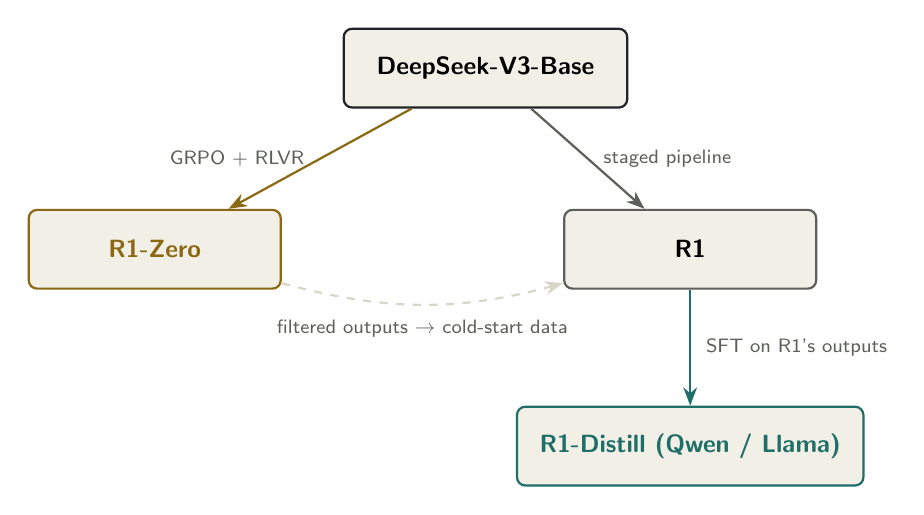
\begin{tikzpicture}[>=Stealth, font=\sffamily]
 \tikzstyle{basenode}=[rectangle,rounded corners=3pt,draw=ink,thick,fill=panel,minimum width=3.6cm,minimum height=1cm,align=center,font=\small\bfseries]
 \tikzstyle{zeronode}=[rectangle,rounded corners=3pt,draw=accent,thick,fill=panel,minimum width=3.2cm,minimum height=1cm,align=center,font=\small\bfseries,text=accent]
 \tikzstyle{r1node}=[rectangle,rounded corners=3pt,draw=inkdim,thick,fill=panel,minimum width=3.2cm,minimum height=1cm,align=center,font=\small\bfseries]
 \tikzstyle{distillnode}=[rectangle,rounded corners=3pt,draw=accentB,thick,fill=panel,minimum width=4.4cm,minimum height=1cm,align=center,font=\small\bfseries,text=accentB]
 \tikzstyle{lbl}=[font=\scriptsize\sffamily,text=inkdim,align=center]
 \node[basenode] (base) at (0,0) {DeepSeek-V3-Base};
 \node[zeronode] (zero) at (-4.2,-2.3) {R1-Zero};
 \node[r1node] (r1) at (2.6,-2.3) {R1};
 \node[distillnode] (distill) at (2.6,-4.8) {R1-Distill (Qwen / Llama)};
 \draw[->,accent,thick] (base) -- node[lbl,left,xshift=-2pt]{GRPO + RLVR} (zero);
 \draw[->,inkdim,thick] (base) -- node[lbl,right,xshift=2pt]{staged pipeline} (r1);
 \draw[->,linecol,thick,dashed] (zero) to[bend right=15] node[lbl,below,yshift=-2pt]{filtered outputs $\rightarrow$ cold-start data} (r1);
 \draw[->,accentB,thick] (r1) -- node[lbl,right,xshift=2pt]{SFT on R1's outputs} (distill);
\end{tikzpicture}
}
\end{center}
{\small\color{ink}Solid arrows are real training --- new weights come out the other end. The dashed arrow is data only: R1-Zero's filtered outputs feed R1's training set, but R1's weights never come from R1-Zero's checkpoint.}
\end{frame}

% ================= 24 : IMPLEMENTATION =================
\begin{frame}[fragile]
\eyebrow{Implementation \textperiodcentered\ 36}{\S7.8\,--\,7.10}
\headline{One scalar loss, one backward pass}
\begin{eqbox}
$L(\theta) = -A\sum_{t=1}^{T}\log\pi_\theta(a_t|s_t)$
\end{eqbox}
\begin{lstlisting}
# log_probs holds one term per generated token
loss = -advantage * log_probs.sum()
loss.backward()
optimizer.step()
\end{lstlisting}
{\small\color{ink}\texttt{backward()} does not need to be called per token. Differentiation is linear, so autograd accumulates every token's gradient contribution into one computation graph automatically.}
\par\vspace{6pt}
\begin{callout}
\clabel{accentB}{The short version}
{\small\color{ink}Same principle as minibatch SGD: sum the per-example losses into one scalar, then call \texttt{backward()} once.}
\end{callout}
\end{frame}

% ================= 25 : SUMMARY =================
\begin{frame}
\eyebrow{Close \textperiodcentered\ 37}{\S7.15}
\headline{The whole lineage, one line each}
\small
\renewcommand{\arraystretch}{1.25}
\begin{tabular}{@{} l p{12.8cm} @{}}
{\bfseries\color{accent}REINFORCE} & Reinforce every sampled token by how well the whole response scored. \\
{\bfseries\color{accent}+ baseline} & Compare against what's typically expected, not the raw score. \\
{\bfseries\color{accent}PPO} & The baseline is a learned value model; KL is baked into the reward; updates are clipped. \\
{\bfseries\color{accent}GRPO} & The baseline is the average of a sampled group; KL is its own loss term; no critic to train. \\
{\bfseries\color{accent}GRPO + RLVR} & For verifiable tasks, even the reward itself comes from a deterministic checker. \\
\end{tabular}
\par\vspace{16pt}
\begin{calloutwarm}
\clabel{accent}{The one idea underneath all of it}
{\normalsize\color{ink}Every step nudges sampled tokens up or down by how good they were relative to expectation. What changes, each time, is only where ``expectation'' comes from.}
\end{calloutwarm}
\end{frame}

\end{document}
